%% Signale.tex
%% $Id: Signale.tex 4 2005-10-10 20:51:21Z bless $
%%

Das Kapitel \textbf{Implementierung} wird anhand dem im Entwurf besprochenen Verlauf der Studie erkl{\"a}rt.

Bei der Entwicklung des Programms hat man sich Gedanken {\"u}ber ein System gemacht, bei dem man alle Daten schon digital abgespeichert hat und nicht noch Informationen vom Probanden von Fragebögen per Hand in den PC eintragen muss. Aus diesem Grund hat man sich f{\"u}r eine Grafische Benutzeroberfl{\"a}che, auch kurz GUI (graphical user interface) genannt, entschieden. 
Die Programmiersprache die verwendet wurde ist C\# gewesen.
Der Entstehungsprozess wurde auf Papier entworfen. Das Design sollte schlicht und einfach sein und den Fokus auf das Programm und nicht auf andere Komponenten des Betriebsystems ablenken. Die Papier Skizzen sind im Anhang vorhanden.

\paragraph{Informationen zur Person}

\begin{figure}[htbp] 
	\centering
	\begin{minipage}[t]{0.45\textwidth}
		\includegraphics[width=\textwidth]{pics/gui/{AngabenZurPerson1}.png}
	\end{minipage}
	\begin{minipage}[t]{0.45\textwidth}
		\includegraphics[width=\textwidth]{pics/gui/{AngabenZurPerson2}.png}
	\end{minipage}
	\caption{GUI f{\"u}r die Befragung zu den Angaben zur Person}
	\label{fig:AngabenZurPerson}
\end{figure}

Bei den Nachforschungen des Studiendesigns \cite{benyon2005designing}, habe man sich nach mehreren Entw{\"u}rfen f{\"u}r folgende Fragen entschieden:

\begin{itemize}
\item Wie alt sind Sie?
\item Angabe des Geschlechts
\item Empfinden Sie sich als musikalisch? 
\item Spielen Sie gelegentlich Computer Spiele?
\item Haben Sie Erfahrungen mit Taktilen Ger{\"a}ten?
\item Haben Sie schon einmal eine Smartwatch verwendet?
\end{itemize}

Da man f{\"u}r den Probanden nicht mit allen Fragen auf einmal {\"u}berh{\"a}ufen wollte, hat man diese Fragen auf zwei Seiten dargestellt \autoref{fig:AngabenZurPerson}. Bei der Frage um das Geschlecht habe man ebenfalls drei antwortmöglichkeiten geboten, ob man \textit{männlich}, \textit{weiblich} oder \textit{keine Angabe}.
Im Hintergrund hatte man eine einfache Klasse \textbf{Person}, die die Informationen der Antworten dieser Befragung gespeichert hat. Um zu vermeiden, dass Daten verloren gehen, habe man die Daten zur Person schon nach diesem Schritt in einer externen Datei gespeichert. F{\"u}r jeden Probanden hat man im Vorfeld eine anonymisierte Datei angelegt, die im Nachhinein nicht mehr auf den Probanden zur{\"u}ckschlie{\ss}en konnte.  

\paragraph{Signal}
Wie schon im Entwurf beschrieben, ist das Signal eines der wichtigsten Bestandteile des Programms.
%Das Signal ist wie im Entwurf schon beschrieben, einer der wichtigsten Bestandteile meines Programms. 

Ein \textbf{Signal} besitzt die Attribute L{\"a}nge in ms, St{\"a}rke, die den jeweiligen Zustand der St{\"a}rke speichert \autoref{fig:zdiagramm}, den Signaltypen, sowie die Grenzen des Signaltypens und die Anzahl wie oft ein Signal erneut abgespielt wurde. 
Da man in den n{\"a}chsten beiden Phasen dem Signal einen Signaltypen zuordnen soll, wurde daf{\"u}r auch ein weiteres Attribut angelegt, sowie die Zeit, die ben{\"o}tigt wurde um die Frage zu beantworten.
%Jedes Signal beinhaltet die Attribute L{\"a}nge, St{\"a}rke, der Signaltyp sowie die Grenzen des Signaltyps.

In der Phase indem der Algorithmus durchgef{\"u}hrt wird, werden noch zwei zus{\"a}tzliche Fragen gestellt f{\"u}r die man in der Klasse \textbf{Signal} auch noch diese beiden Werte gespeichert hat.

%Je nach dem in welcher Phase des Programms man sich gerade befindet, werden noch weitere Attribute gespeichert
%Das Programm besteht aus vier Phasen.

\paragraph {Bestimmung der Grenzen durch Bewertung durch den Nutzer}

\begin{figure}
	\centering
    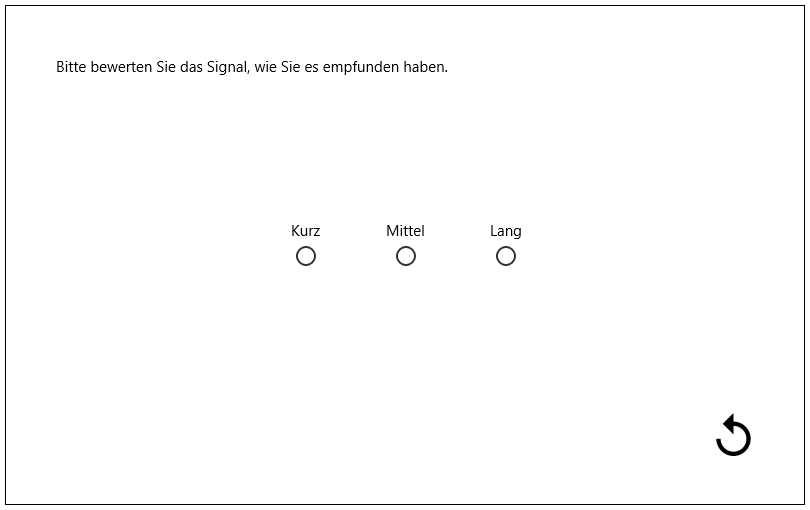
\includegraphics[width=\textwidth]{pics/gui/GrenzenBestimmen.png}
    \caption{GUI zur Bestimmung der Grenzen}
    \label{fig:GrenzenBestimmen}
\end{figure}

Nachdem der Proband die Angaben zur Person beantwortet hat, erscheint ein Benachrichtigungsfenster, indem Informationen {\"u}ber den die aktuelle Phase erkl{\"a}rt wird. 
Falls der Proband zu einem Zeipunkt Fragen haben sollte, werden diese durch den Aufseher beantwortet.
F{\"u}r die Bestimmung der Grenzen wurden 10 Signale erzeugt, die gleichverteilt sind. 
Mithilfe einer Zufallsfunktion werden diese Signale zuf{\"a}llig ausgew{\"a}hlt und in dieser Reihefolge abgespielt. 
Der Proband soll f{\"u}r jeden der 10 Signalen einen der Signaltypen \textit{Kurz}, \textit{Mittel} oder \textit{Lang} zuordnen. 
Dabei habe man die im Entwurf besprochenen Sonderf{\"a}lle {\"u}berpr{\"u}ft und bei erfolgreicher Bildung der Grenzen ist man in die n{\"a}chste Phase {\"u}bergegangen.
%Als alle 10 Signale bewertet wurden, hat man {\"u}berpr{\"u}ft, ob der Kleinste Wert von 100ms Kurz und der gr{\"o}{\ss}te Wert von 1000ms Lang gewesen ist. 

Wenn die Bestimmung der Grenzen nicht erolgreich gewesen ist, wird der Benutzer gebeten die gleiche zuf{\"a}llige Reihenfolge erneut zu bewerten. 

Sollte ein Proband den Replay-Button dr{\"u}cken, wird das letzte Signal erneut abgespielt.

F{\"u}r die GUI \autoref{fig:GrenzenBestimmen} hat man sich auf das wesentliche beschr{\"a}nkt. Die Anweisung an den Benutzer war immer die selbe, daher hat man nur den gleichen Text dargestelllt. Als Antwortm{\"o}glichkeiten des Signals wurde für jeden Sognaltyp je ein Radio-Button erstellt. 
In den Phasen, in denen ein Signal abgespielt wurde, wurde der Replay-Button immer an der gleichen feste Position plaziert. 

Der Ablauf einer Bewertung wird im folgenden beschrieben. Nach der Best{\"a}tigung des Benachrichtigungsfenster wurden im Hintergrund die 10 Signale in zuf{\"a}lliger Reihenfolge ausgew{\"a}hlt. Darauf wurde das erste Signal {\"u}ber BLE an das Wearable gesendet. Das Wearable hat dieses Signal empfangen, ausgewertet und hat die Informationen als Vibration abgespielt. Das was der Benutzer dadurch empfunden hat wurde {\"u}ber den PC mittels der Maus bewertet. Nach einer Bewertung gab es keine M{\"o}glichkeit die Bewertung eines vorherigen Signals erneut anzupassen. Nachdem das Signal vom Probanden bewertet wurde, wurde der Maus-Cursor durch dem Programm an eine Anfangsposition gesetzt, damit der Benutzer nicht unabsichtlich doppelt auf ein Radio-Button dr{\"u}cken konnte. Um dem Probanden zu signalisieren, dass er die Checkbox gedr{\"u}ckt hat, hat man die Check-Box einen Augenblick visuell markiert gelassen, nachdem man den Maus-Cursor neu positioniert hat. Mit der Neupositionierung der Maus hat man erreicht, dass man immer den gleichen Weg hatte um die Checkboxen zu erreichen, aber man hatte auch nach mehreren Fragen die Maus anheben weiter nach oben legen m{\"u}ssen, denn man hat schon das Ende der Tischkannte erreicht. Nach einer Bewertung wurde die vorherige Auswahl entfernt und man hat das n{\"a}chste Signal {\"u}bertragen.

\paragraph {3. Ausf{\"u}hren des Algorithmus}

\begin{figure}[htbp] 
	\centering
	\begin{minipage}[t]{0.45\textwidth}
		\includegraphics[width=\textwidth]{pics/gui/{Algorithmus1}.png}
	\end{minipage}
	\begin{minipage}[t]{0.45\textwidth}
		\includegraphics[width=\textwidth]{pics/gui/{Algorithmus2Emotion}.png}
	\end{minipage}
	\caption{GUI des Algorithmus (links) und der Bewertung der Stimmung (rechts)}
	\label{fig:AlgorithmusBild}
\end{figure}

Für den Algorithmus habe man sich mehrere Klassen erzeugt. 
Die Klasse \textbf{DNA} beinhaltet ein Signal und Hilfsfunktionen, die eine Rekombination und eine Muatation von zwei Signalen erzeugen.
In der Klasse \textbf{Population} hat man eine Liste aus 30 Elementen, von einer Klasse \textbf{DNA} erstellt, dabei sind beinhalten die ersten 10 DNA-Objekte Signale, die den Signaltypen \textit{Kurz} haben. Für die nachfolgenden DNA-Objekte gilt das selbe nur mit \textit{Mittel} gefolgt von \textit{Lang}. 
Bei der Erzeugung der Signale habe man mittels einer Zufallsfunktion sich Signale mit einer zufälligen Stärke und einer zufälligen Länge zwischen den Grenzen des jeweiligen Signaltypens erstellt. Beim ersten Aufruf der Klasse \textit{Population} habe man die Grenzen der Signaltypen ebenfalls als ein Signal erzeugt und in der Liste hinzugefügt.

Für die Grafische Benutzeroberfläche hat man sich für die drei folgenden Fragen entschieden:
\begin{itemize}
\item Was für einen Signaltypen haben Sie erkannt?
\item Wie gut haben Sie das Signal erkannt?
\item Wie empfanden Sie die Stärke des Signals?
\end{itemize}

Es ist bis auf die Anzahl der Fragen genau das gleiche Prozedere gewesen. Es wurde zuerst ein Erklärungsfenster dargestellt, so dass der Benutzer weiß, was in dieser Phase von Ihm erwartet wird. 
Dabei wird im Hintergrund wie gerade erwähnt eine Population erzeugt. Diese Population wird DNA für DNA abgearbeitet. Dabei wird für jede DNA enthaltene Signal über BLE an das Wearable gesendet und die Information in Vibration umgewandelt. Dabei hat der Benutzer die drei Fragen zu dem Signal beantworten sollen. 
Es musste die komplette Population bewertet werden, es wurde keine DNA erneut bewertet. Man habe dabei zufällig eine DNA aus der Population gewählt, die bewertet werden sollte.

Die erste Frage diente nur dazu um in der späteren Auswertung herauszufinden, was der Benutzer im Vergleich zum Programm erkannt hat. 
Die zweite Frage wurde als eigentlicher Fitnesswert gespeichert. Die Repräsentation der Frage ist in der Tabelle \autoref{} zu sehen.
Die Stärke wurde direkt nach der Beantwortung aller drei Fragen nach dem Zustandsdiagramm verändert.

Die Informationen der Stärke und des Fitnesswerts habe man in der Klasse \textit{Signal} noch mitgespiechert.

Nachdem eine Population komplett berechnet wurde, habe man den Generations-zähler um eins erhöht, die bisherigen Informationen in der externen Datei gespeichert und eine neue Population aus den Werten erzeugt.

%Die Erzeugung ist dabei so vonstatten gegangen:...
\paragraph{Selektion}
Für jeden Signaltypen hat man einen Pool aus DNA-Objekten erstellt, dessen Signale den jeweiligen Signaltypen besitzen.
Anhand der Formel X (im Entwurf) habe man eine Anzahl berechnet, wie oft ein DNA-Objekt in das jeweilige Pool hinzugefügt wird. Im Schnitt hatte man nach dem Hinzugügen aller DNA-Objekte knapp 1000 Elemente in einem der Pools. 

\paragraph{Rekombination}
Bei der Rekombination verwendet man 




%\paragraph {1. Aufnahme der Personalien}
%Der erste Schritt bestand darin, den Probanden den Personalien zu fragen. 

%\paragraph {2. Bestimmung der Grenzen durch Bewertung durch den Nutzer}
%\paragraph {3. Ausf{\"u}hren des Algorithmus}
\paragraph {4. Muster Erkennung} 

%Das Signal ist ein wichtiger Bestandteil meines Programm. 
Ein Signal beinhaltet die Signall{\"a}nge, die in Millisekunden gespeichert wird, und eine Signalst{\"a}rke, die in 5 St{\"a}rkestufen eingeteilt ist. 



Ich habe meinen Evolution{\"a}ren Algorithmus so angepasst, dass bei mir ein Induviduum ein Signal ist. 
Ich habe dem Benutzer das Signal mit dem Wearable abspielen lassen und im Anschluss Fragen beantworten lassen. 
Er sollte bewerten wie gut er das Signal erkannt hat. Die Bewertung vom Benutzer war entscheidend um nach der kompletten Bewertung der Population 

% -----------------------------------------------------------------------

%\paragraph {1. Aufnahme der Personalien}


%Um in der Evaluierung m{\"o}gliche Erkentnisse zwischen bestimmten Benutzergruppen herausfinden zu k{\"o}nnen, hat man dem Benutzer Eine Reihe von Fragen gestellt, die im Bild XXXX zu sehen sind.
%Diese Daten wurden anonymisiert gespeichert. 

%\paragraph {2. Bestimmung der Grenzen durch Bewertung durch den Nutzer}


%\paragraph {3. Ausf{\"u}hren des Algorithmus}


%\paragraph {4. Muster Erkennung} 

%MUSTER BILD

